\chapter{Dokumentace}

\section{Vstupní data}

Jak jsme již zmiňovali, naše knihovna využívá výstupní data nástroje Traveler
jako vstupní data. Jedná se o data ve formátu JSON, obsahující všechny potřebné
informace o rozložení nukleotidů, jejich párování, velikostech popisků, barvách
a tlouštkách čar. Kromě informací o rozložení obsahuje také informace o
potřebných editacích vzorové sekundární struktury.

V rámci R2DT projektu vzníká i JSON
schéma\footnote{https://github.com/LDWLab/RNA2D-data-schema}, které by mělo
popisovat strukturu vstupních dat. Schéma je stále ve vývoji, proto aktuální
výstupy R2DT nebo Traveleru neodpovídájí schématu a je dost možné, že se jejich
výstupy budou v budoucnu měnit a naše knihovna se jim bude přizpůsobovat,
{\color{red}TODO: přepsat}protože RNAcentral, využívající R2DT, je největší databází s
2D RNA strukturama.

Samotná struktura dat není složitá, ale popíšeme zde pouze tu část, kterou
aktuálně využíváme, kromě toho, že ostatní data pro nás nejsou duležitá, tak
jak již bylo zmíněno samotná struktura dat není pevně daná a může se měnit.

Jedná se o objekt, který má dvě položky - \texttt{classes}, což je pole objektů
popisující třídy říkající způsob zobrazení struktury, podobně jako to kaskádové
styly (CSS) diktují pro webové stránky a \texttt{rnaComplexes}. 

\texttt{rnaComplexes} je pole polí sloužící pro popis celých skupin RNA
struktur. Naše knihovna pracuje vždy pouze s nultým prvkem. Neviděli jsme důvod
to dělat jinak, a pokud by se nějaký důvod našel v budoucnu, neměl by být
problém naší knihovnu přizpůsobit situaci (např. rozšířením o novou metodu pro
zachování zpětné kompatibility).

V rámci naší knihovny jsme vytvořili interface, který vstupní data musí
splňovat. Struktura zbytku dat by měla být jasně viditelná z následujícího
diagramu těchto interfaceů.

\begin{figure}[H]
  \centering
  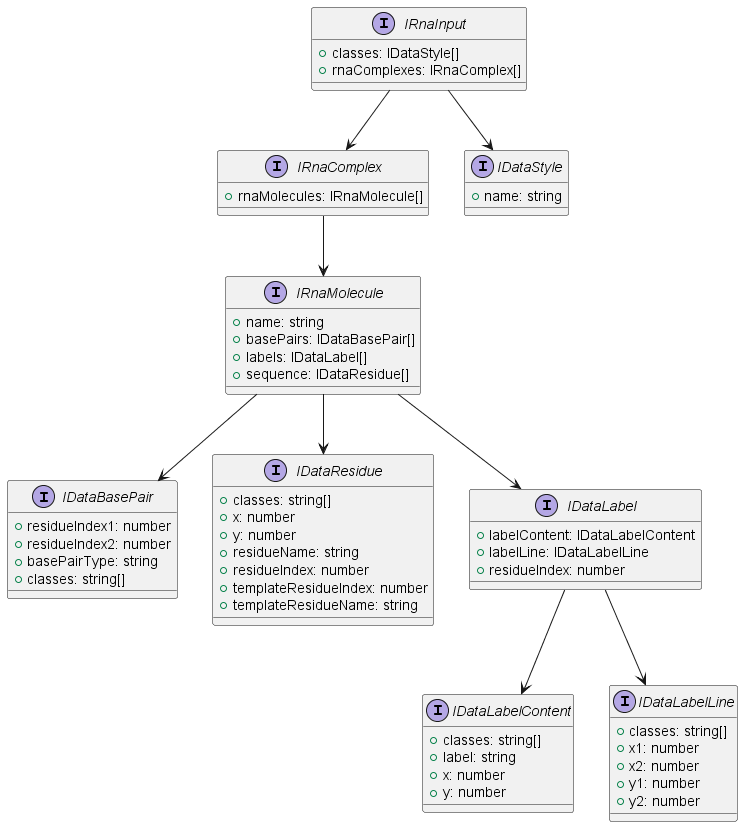
\includegraphics[width=145mm]{../img/kap03/rnaInput.png}
  \caption{Interface pro vstupní data}
\end{figure}

Při vykreslení dat si můžeme všimnout různého obarvení jednotlivých residue.
Tyto barvy slouží k lepšímu zorientování ve struktuře vzhledem ke vzorové
struktuře. Černá barva značí, že residue leží na poloze vzorového residue se
stejným názvem. Zelenou barvou jsou označený ty residue jejiž vzorový residue
bylo třeba přejmenovat. Modrou barvou jsou vyznačený posunutý residue. A poslední
růžovou barvu mají nově přidaný residue.

\begin{figure}[H]
  \centering
  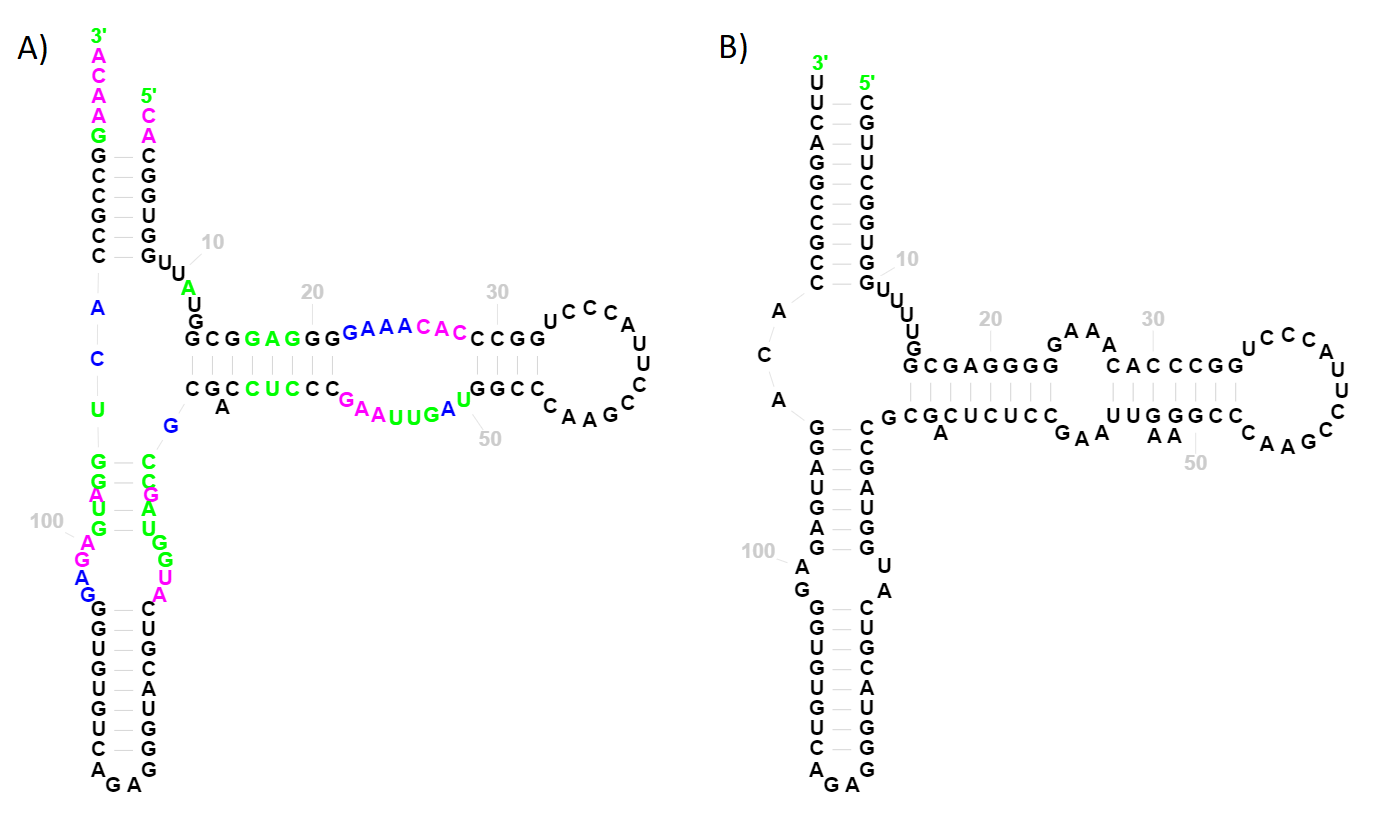
\includegraphics[width=140mm]{../img/kap03/inputDataColors.png}
  \caption{A) Odvozená sekundární RNA struktura URS00000B9D9D\_471852, B)
  Vzorová sekundární RNA struktura d.5.b.A.madurae}
\end{figure}

\section{Objektový návrh}

Udělat dobrý objektový návrh je pro knihovnu, která má usnadňovat práci velmi
důležité, zároveň je tento úkol velmi těžký, speciálně v případě kdy není
předem jasné, co všechno má knihovna umět. To v našem případě nebylo, a proto
se některá rozhodnutí mohou zdát zpětně zvláštní, při nejmnenším ne ideální.

{\color{red}TODO: přepsat}V následující kapitole se pokusíme čtenáře seznámit s
objektovým návrhem naší knihovny včetně s myšlenkama, které nás k takovému
návrhu dovedli. Nejdříve dáme čtenáři obecný pohled na strukturu a následně
rozebere jednotlivé třídy podrobněji.

\subsection{Obecný pohled na třídy}

Srdcem celé knihovny je třída \texttt{RnaVis}, která vykresluje struktury na
canvas a nastavuje se přes ní zoom/panning. Kromě toho má v sobě také uložené
vrstvy realizované třídou \texttt{Layer}, představující jednotlivé struktury.

Pro určení vykreslovacích parametrů (např. font, barva, velikost) objektů  máme
třídu \texttt{Styles}. Před každým vykreslení se zeptáme této třídy na
vykreslovací parametry pro daný objekt.

Poslední důležitou velkou částí jsou animace. Tuto funkcionalitu zpřístupňují
dvě hlavní třídy - \texttt{TranslationAnim}, \texttt{VisibilityAnim}. Obě
implementují interface \texttt{IAnimation}. 

Níže jsou tři diagramy tříd, které dohromady obsahují každou třídu. Diagramama
se snažíme vyjádřit obecnou strukturu, tím pádem pro přehlednost neobsahují
všechny informace - všechny metody, některé privátní vlastnosti a některé
závislosti.
 
\begin{figure}[H]
  \centering
  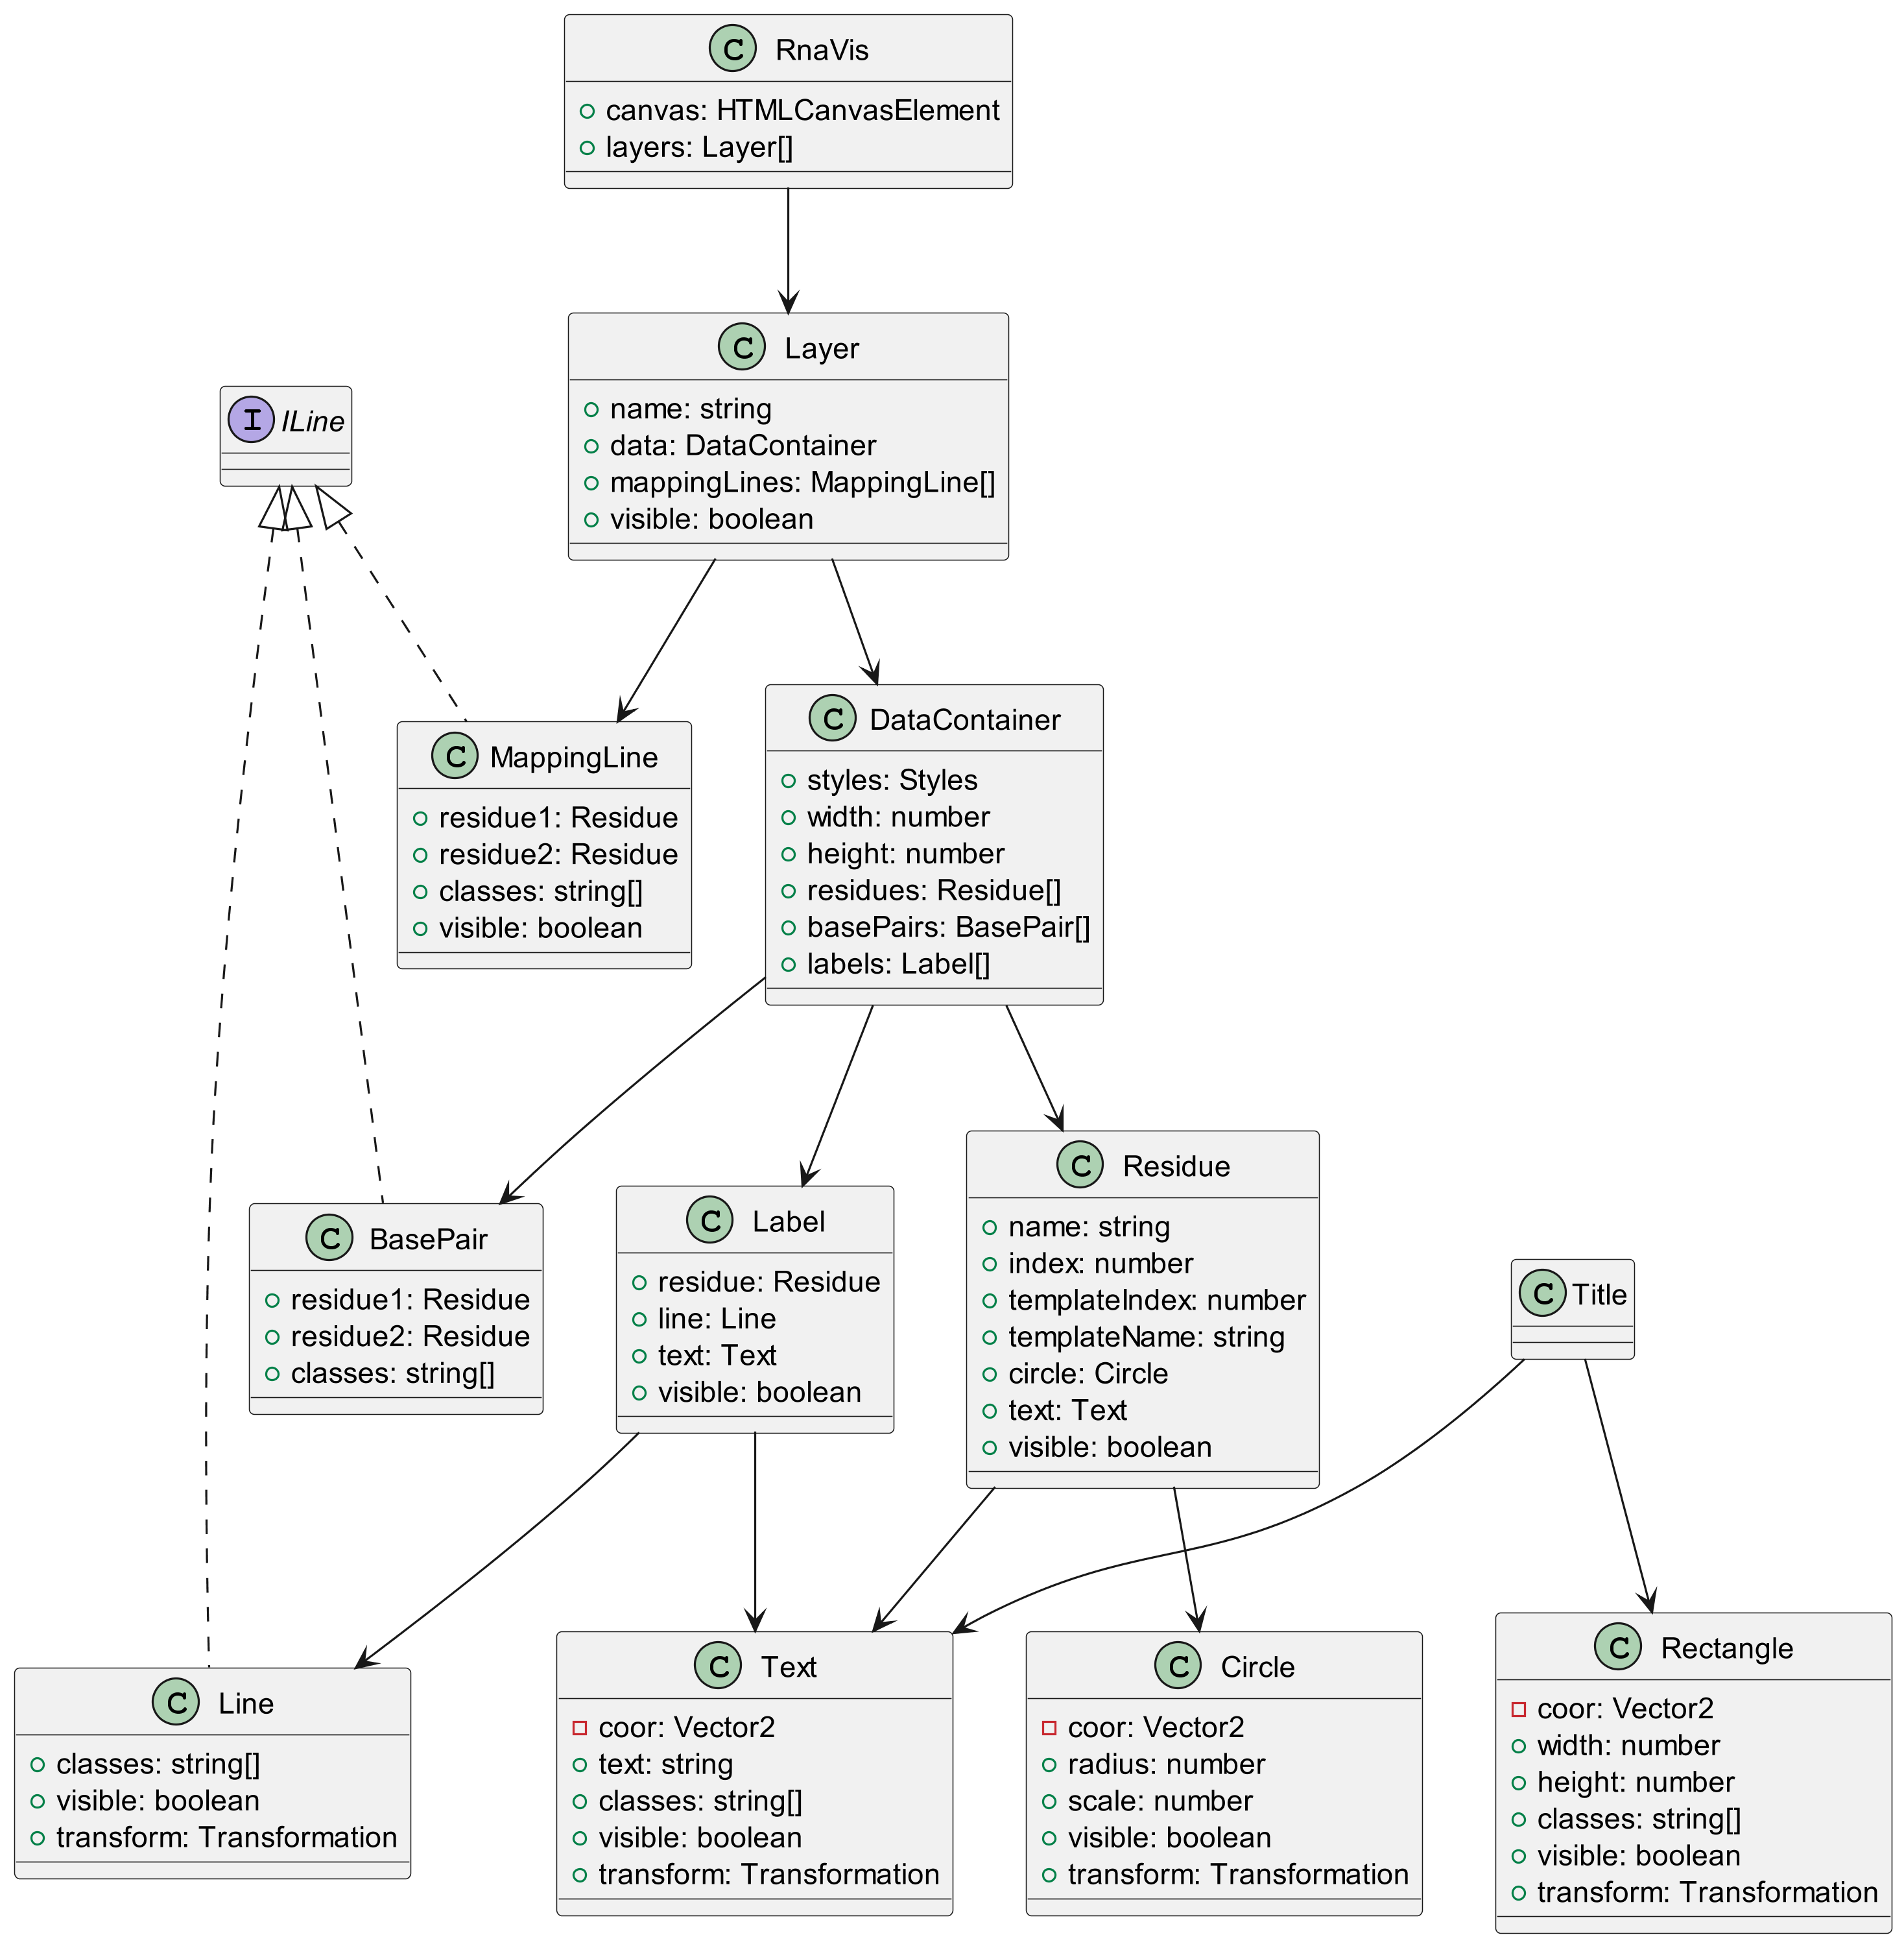
\includegraphics[width=145mm]{../img/kap03/rnavis.png}
  \caption{Diagram tříd}
\end{figure}

\begin{figure}[H]
  \centering
  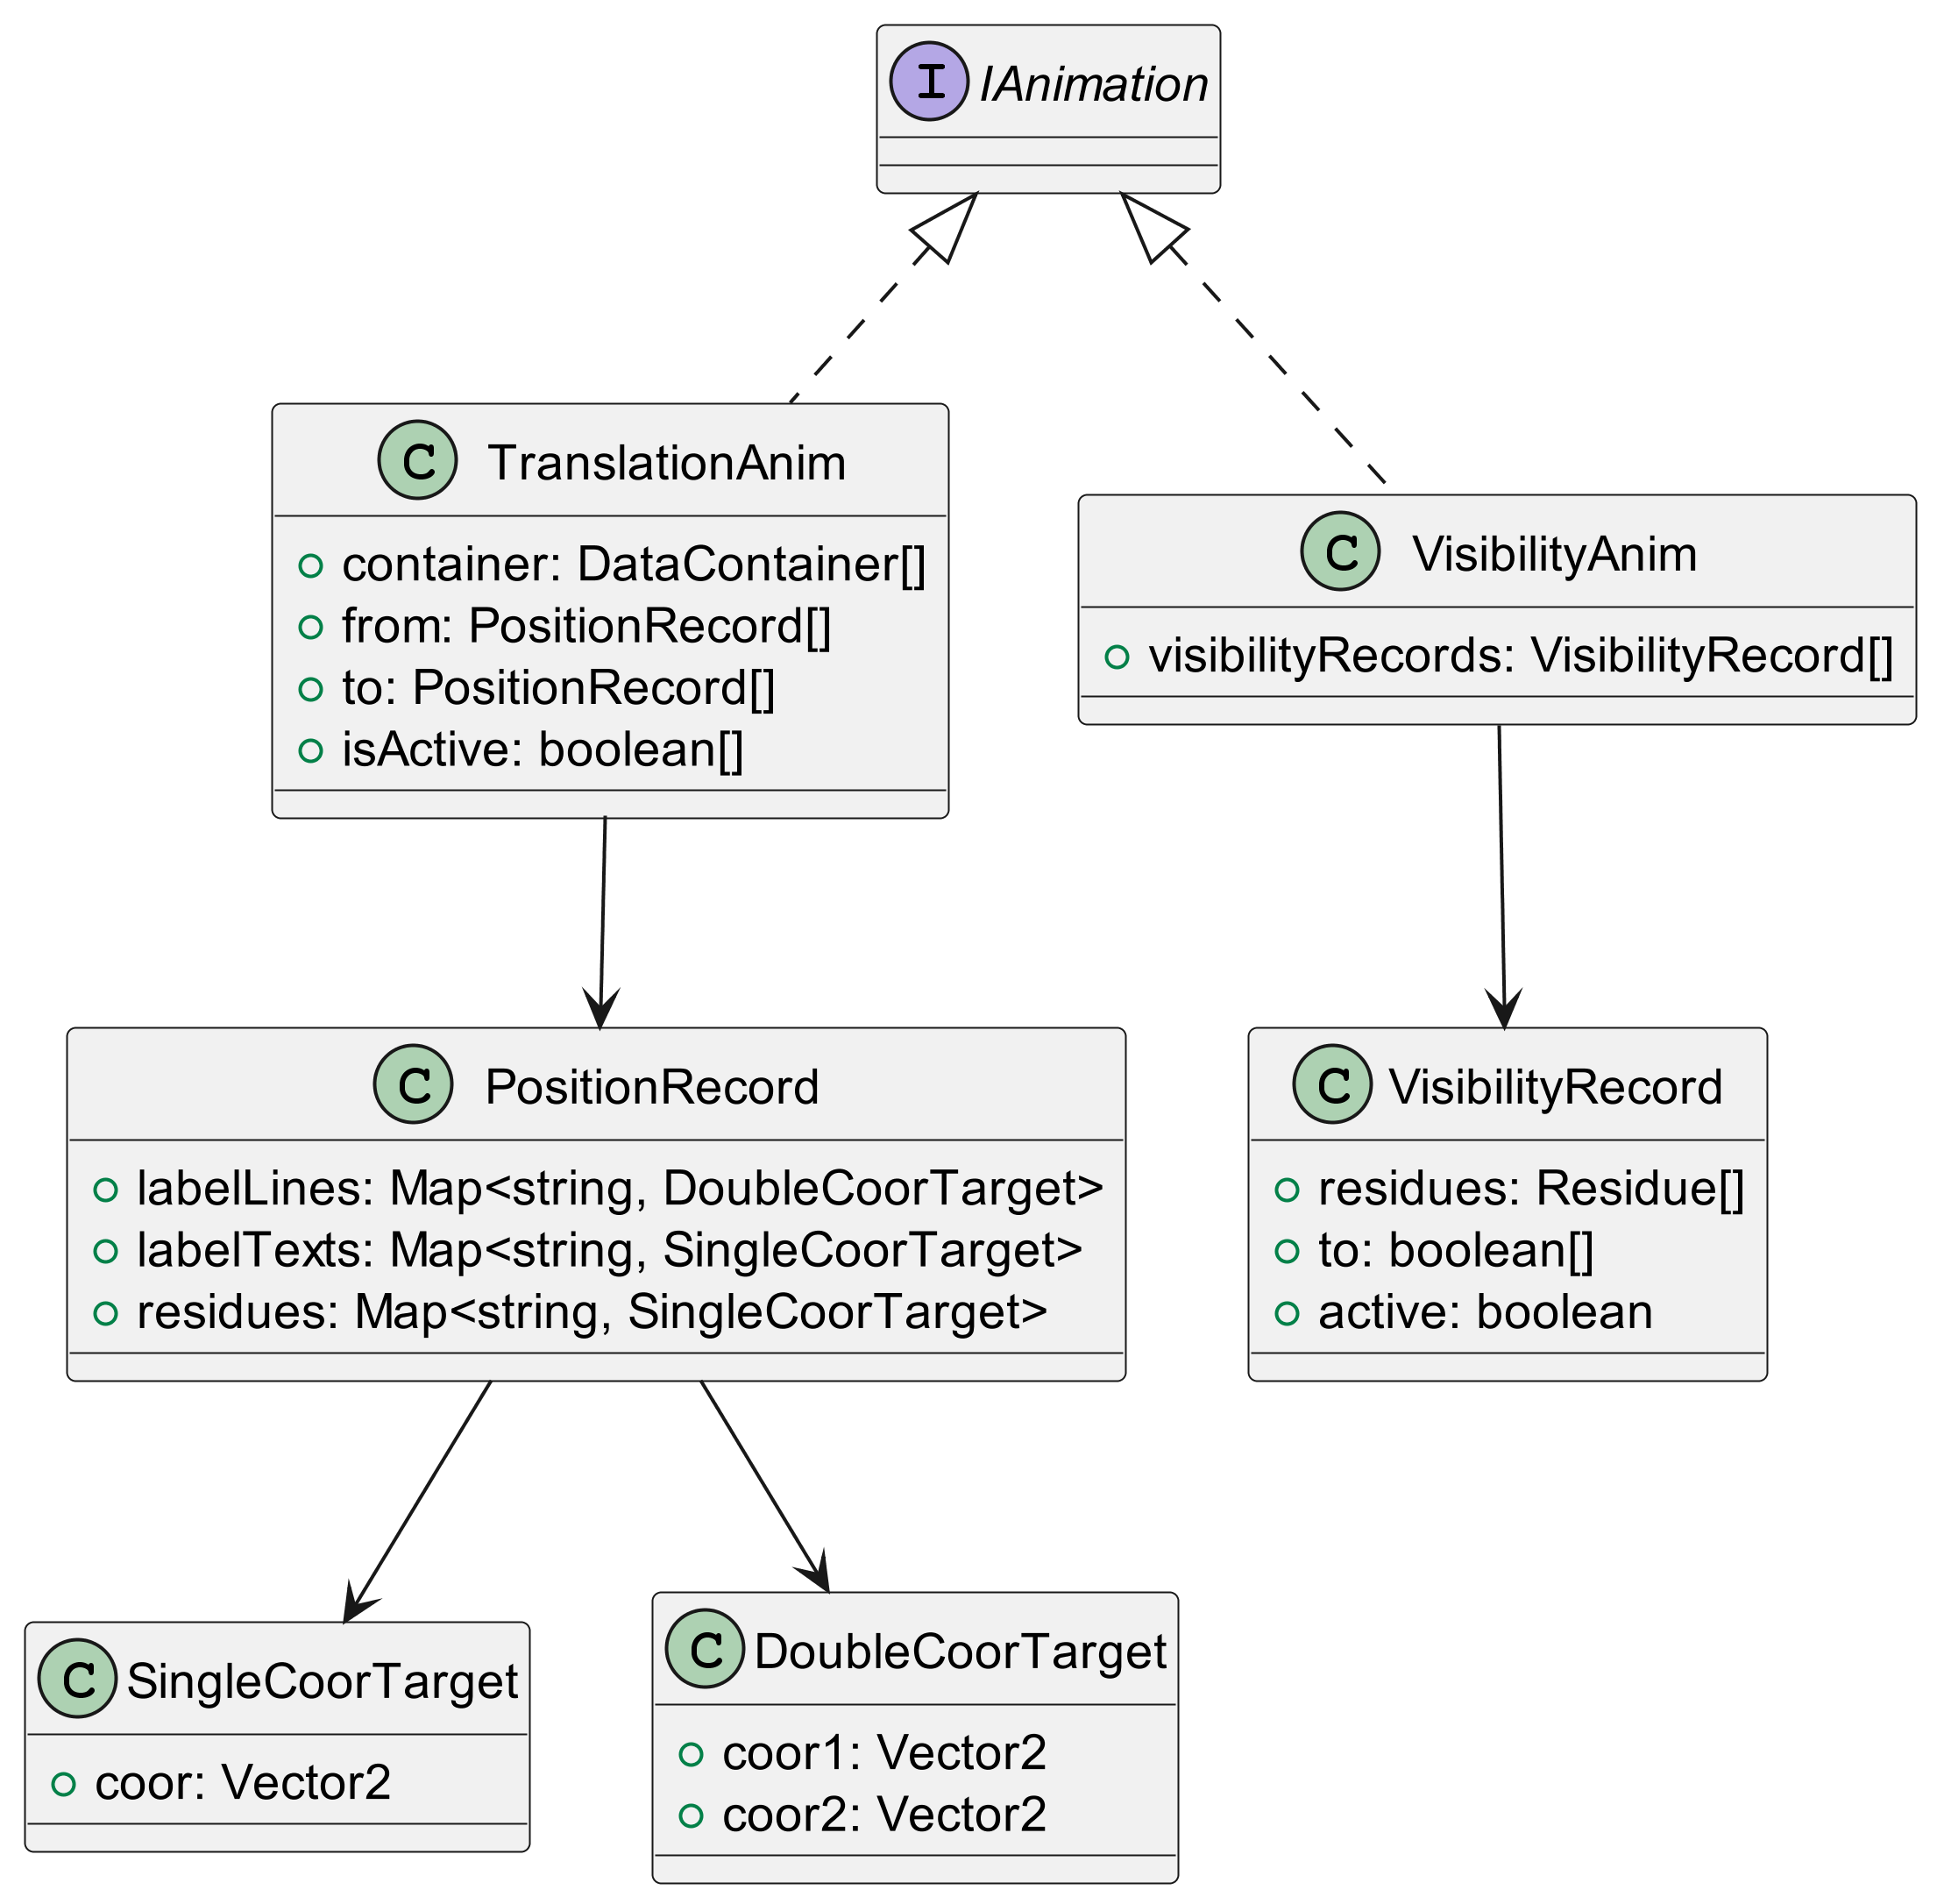
\includegraphics[width=145mm]{../img/kap03/animation.png}
  \caption{Diagram tříd}
\end{figure}

\begin{figure}[H]
  \centering
  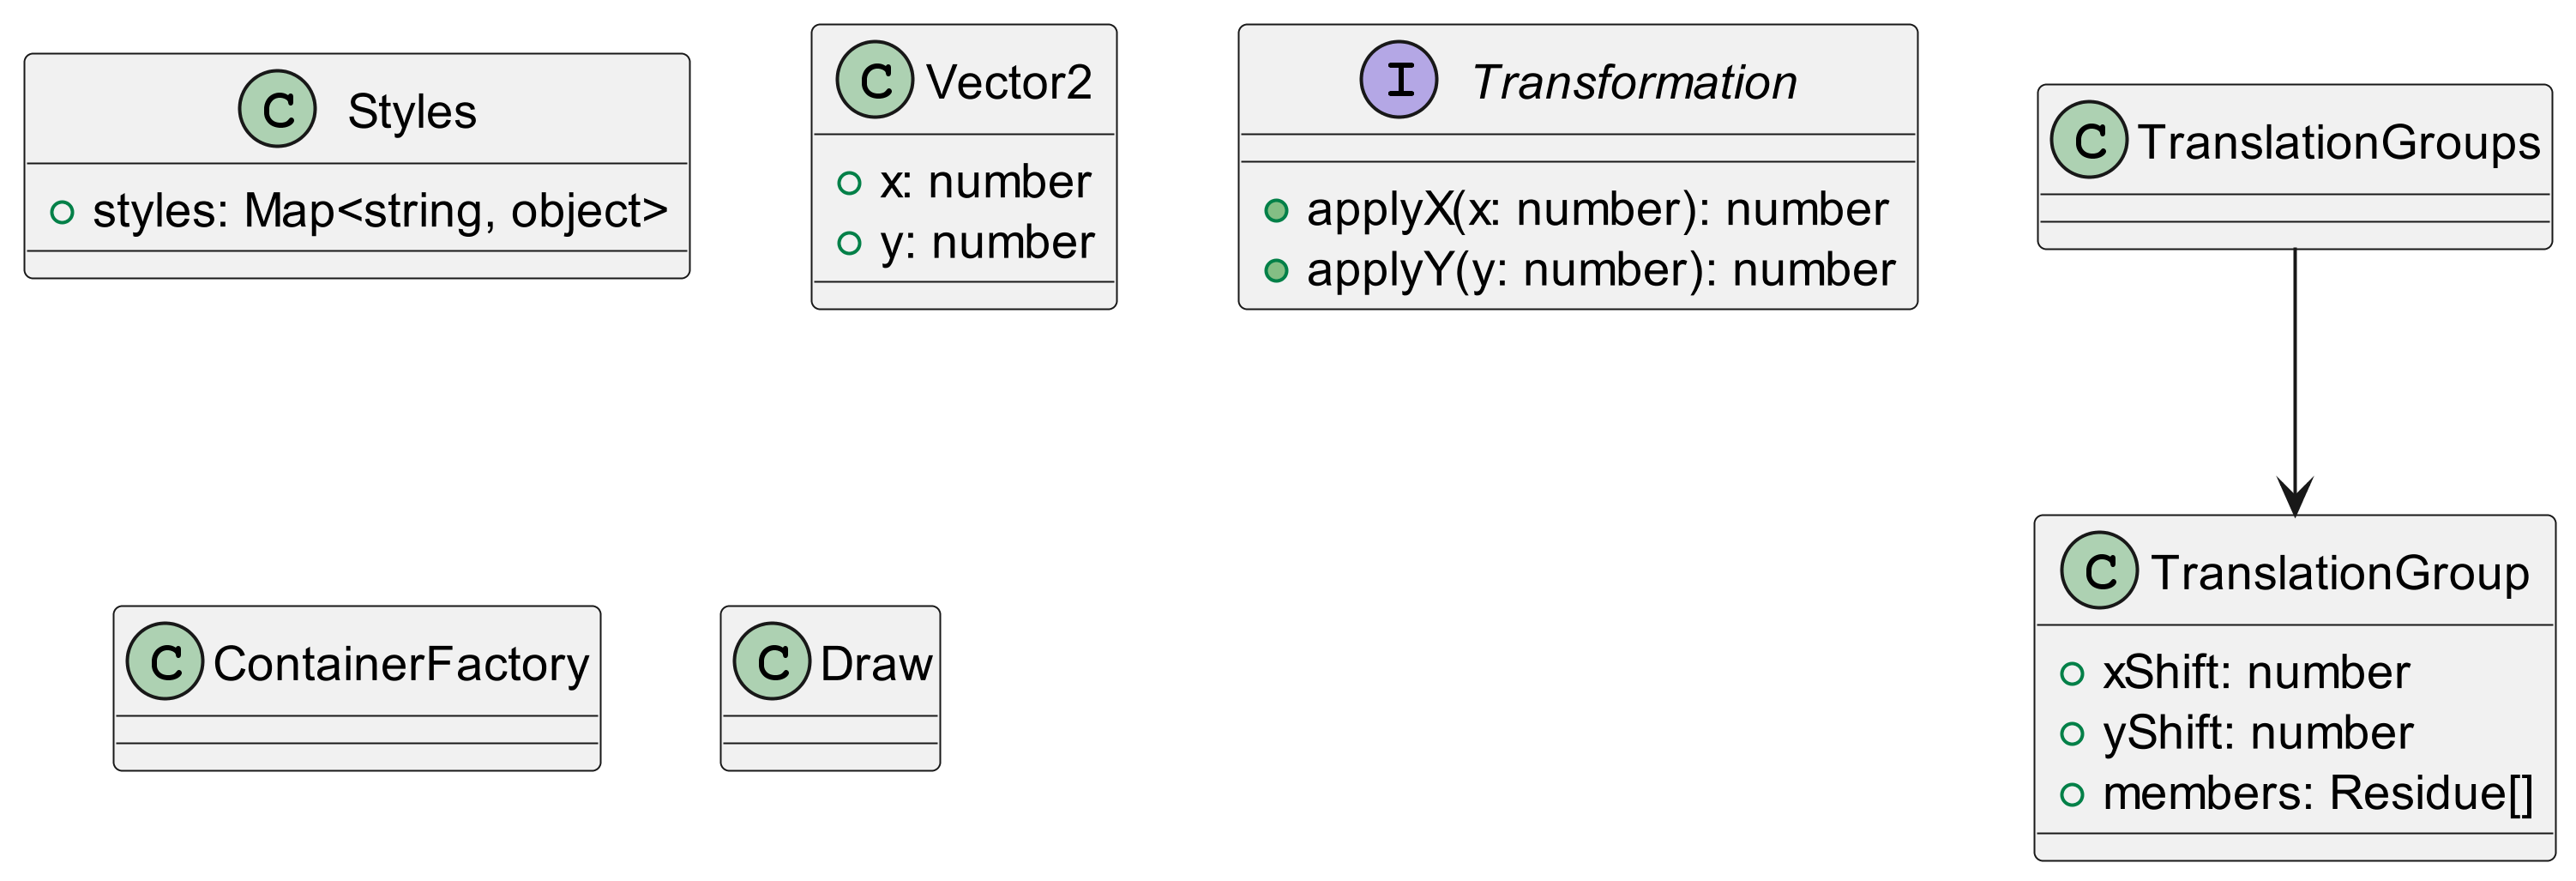
\includegraphics[width=145mm]{../img/kap03/others.png}
  \caption{Diagram tříd}
\end{figure}

\section{Uživatelská dokumentace}

\subsection{Instalace}

\subsection{Rozhraní: IAnimation}

Rozhraní pro definici animace.

\subsubsection{Implementováno}

\begin{itemize}
  \item \texttt{TranslationAnim}
  \item \texttt{VisibilityAnim}
\end{itemize}

\subsubsection{Metody}

\paragraph{animate}\mbox{}\\

\texttt{animate}(rna, duration, after): \texttt{void}

Provede animaci.

\subparagraph{Parametry}\mbox{}\\

\begin{tabular}{|l|l|p{8cm}|}
  \hline
  Název & Typ & Popis \\ \hline
  rna & \texttt{RnaVis} & Objekt RnaVis, na kterém se má animace provést \\ \hline
  duration & \texttt{number} & Délka animace \\ \hline
  after & \texttt{AfterFn} & Funkce, která se má zavolat po dokončení animace \\ \hline
\end{tabular}


\subsection{Příklady}

\subsubsection{Vykreslení struktur}

\subsubsection{Transformace}

\section{Vývojová dokumentace}

\subsection{Volba technologií}

\subsubsection{Programovací jazyk}

Volba programovacího jazyka byla poměrně přímočará. Chtěli jsme napsat
knihovnu, která se bude používat na webu.
Javascript\footnote{https://developer.mozilla.org/en-US/docs/Web/JavaScript} je
v tomto případě jasnou volbou, protože to je v podstatě to jediné, co se
používá. Přesto Javascript není jazyk, ve kterým je naše knihovna psaná,
protože se jedná o dynamicky typovaný jazyk, což s sebou nese určité výhody pro
jednoduché a rychlé psaní kódu, ale u větších projektů se to stává nevýhodou.
Naše knihovna je napsaná v
Typescriptu\footnote{https://www.typescriptlang.org/}, což je nadmnožina
Javascriptu, snažící se řešit jeho slabiny a navíc ho lze snadno přeložit do
Javasrciptu a v této formě distribuovat. Při tomto překladu je možné zachovat i
informaci o konkrétních typech, tím pádem projekty, využívající naší knihovnu,
psané v Typescriptu nejsou ochuzené o typovou kontrolu, kterou typescript
nabízí.

\subsection{Verzování}

Chtěli jsme mít možnost se vracet ke starším verzím projektu v případě, že něco
rozbijeme, nebo by nás pouze zajímali implementace, které už nepoužíváme. Pro
verzování používáme Git\footnote{https://git-scm.com/}, který lze jednoduše
používat s GitHubem\footnote{https://github.com/}. Díky kterému, je náš projekt
přístupný odkukoliv.

Jediným důvodem pro tato rozhodnutí je, že obě technologie známe, nemáme s nimi
problém a neviděli jsme tedy důvod hledat jiné možnosti.

\subsubsection{Knihovna D3.js}

D3.js\footnote{https://d3js.org/} je knihovna v jayzce Javascript pomáhající
přivést data k životu využívající především
SVG\footnote{https://developer.mozilla.org/en-US/docs/Web/SVG} formát, se
kterým se dá v
HTML\footnote{https://developer.mozilla.org/en-US/docs/Learn/Getting\_started\_with\_the\_web/HTML\_basics}
pohodlně pracovat. Její důraz na webové standardy dává uživateli možnost
využívat moderní prohlížeče naplno bez dalších frameworků. S knihovnou není
nejjednodušší se naučit pracovat, ale její velkou předností je rychlost.

\subsubsection{SVG nebo canvas}

V počátcích jsme chtěli k zobrazování používat SVG. Jedná se o webový standard,
který lze skvěle kombinovat s ostatními standardy jako je
CSS\footnote{https://developer.mozilla.org/en-US/docs/Web/CSS},
DOM\footnote{https://developer.mozilla.org/en-US/docs/Web/API/Document\_Object\_Model},
Javascript. V kombinací s D3.js knihovnou je pak dělání animací nebo
aktualizaci stavu SVG objektů jednoduché.

Nebyl důvod SVG nevyužívat, ale později jsme na vlastní kůži pocítili slabinu
SVG. SVG se při vykreslování tisícovek objektů stává velmi pomalé. Takového
počtu objektů můžeme dosáhnout pouze s jednou sekundární RNA strukturou, my
navíc chceme zobrazit více takových struktur a ještě s nimi dynamicky pracovat. 

Tím se pro nás stalo SVG nepoužitelné. Další možností bylo využití
canvasu\footnote{https://developer.mozilla.org/en-US/docs/Web/API/Canvas\_API},
který slibuje výrazně lepší výkon a lze ho stále jednoduše používat.

Některé pro nás klíčové funkce D3.js knihovny lze využít i pro práci s
canvasem. Konkrétně se jedná o zoom, panning a animace.

U canvasu jsme nakonec i zůstali, přestože při práci s desítkama velkých
struktur vykreslování není plynulé.

\subsection{Rozbor implementace}
